The design process for this prototype application consisted of user interface design, android application system design and the activity of choosing resources for a backend host.

\subsection*{User Interface}
The user interface mock ups were created using \parencite{fluid}.
The aim of this design was to provide a simple, easy to use interface so that a user could use the application with minimal effort.
The main benefit of using computer vision for this type of application is to
reduce the effort of the user or dietician keeping track of food intake.
Therefore, this application had to be very quick and easy to use.
The application is called NutriLog.

Three main activities were needed for this application.
The first activity, as seen in Figure \ref{fig:page1}, would consist of options to either take an image of food or to view the food logs of the user.
If the user decides to take an image of food, they will be brought to the second activity which can be seen in Figure \ref{fig:page2}.
The user is required to take a picture before reaching the activity in Figure \ref{fig:page2}.
Once the user presses the send button the image is classified and the content of the activity changes to display the classification and calorie count as in Figure \ref{fig:page3}.
Alternatively, the user can cancel the process and return to the first activity.
The user would then submit the food classification for logging and automatically return to the first activity.
The final activity is displayed when a user views their food logs.
This activity has the ability to view a list of the food logs taken by the user by day, week or month.
The calorie count of the selected time frame is to be displayed on this activity also.

\begin{figure}[h] 
  \label{ fig7} 
  \begin{minipage}[b]{0.5\linewidth}
    \centering
    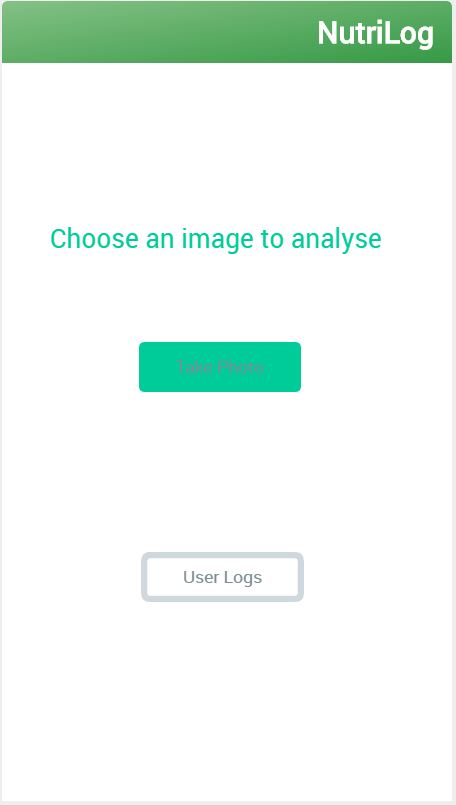
\includegraphics[width=.75\linewidth]{Mockup1} 
    \caption{Landing Activity} 
  \label{fig:page1}
    \vspace{4ex}
  \end{minipage}%%
  \begin{minipage}[b]{0.5\linewidth}
    \centering
    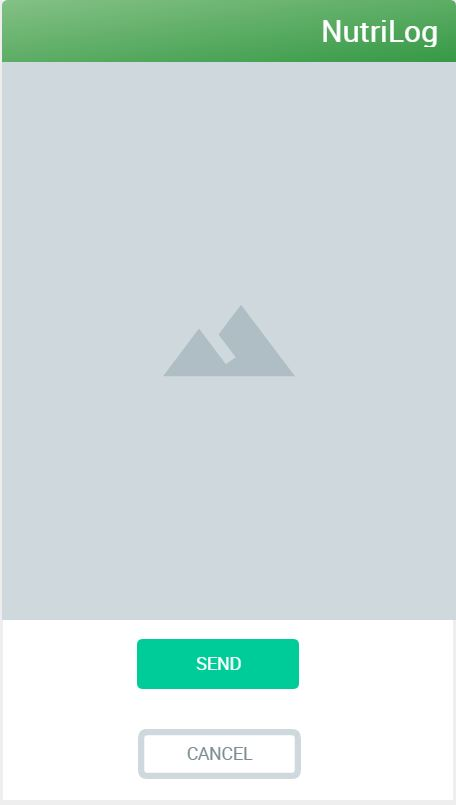
\includegraphics[width=.75\linewidth]{Mockup2} 
    \caption{Image Submission Activity} 
  \label{fig:page2}
    \vspace{4ex}
  \end{minipage} 
  \begin{minipage}[b]{0.5\linewidth}
    \centering
    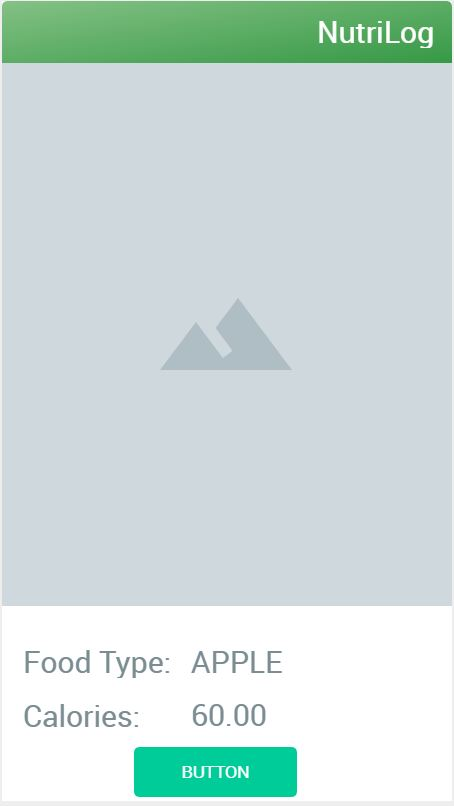
\includegraphics[width=.75\linewidth]{Mockup3} 
    \caption{Classification Activity} 
    \label{fig:page3}
    \vspace{4ex}
  \end{minipage}%% 
  \begin{minipage}[b]{0.5\linewidth}
    \centering
    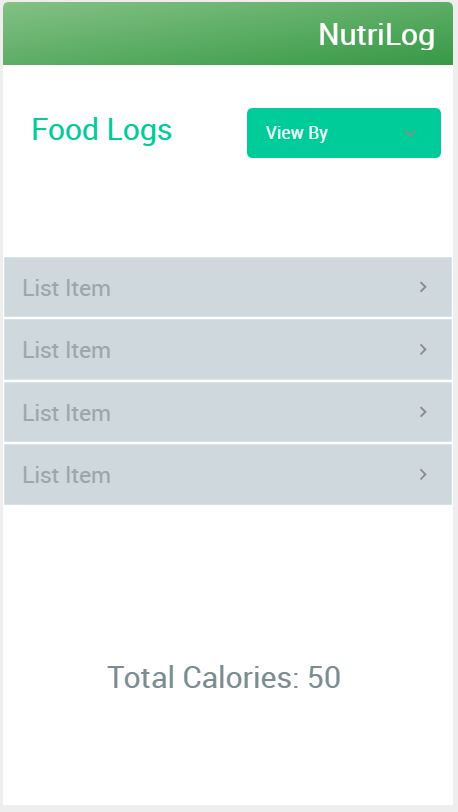
\includegraphics[width=.75\linewidth]{Mockup4} 
    \caption{Food Logs Activity} 
    \label{fig:page4}
    \vspace{4ex}
  \end{minipage} 
\end{figure}
\afterpage{\clearpage}

\subsection*{System Architecture}

\begin{figure}[h]
    \centering
    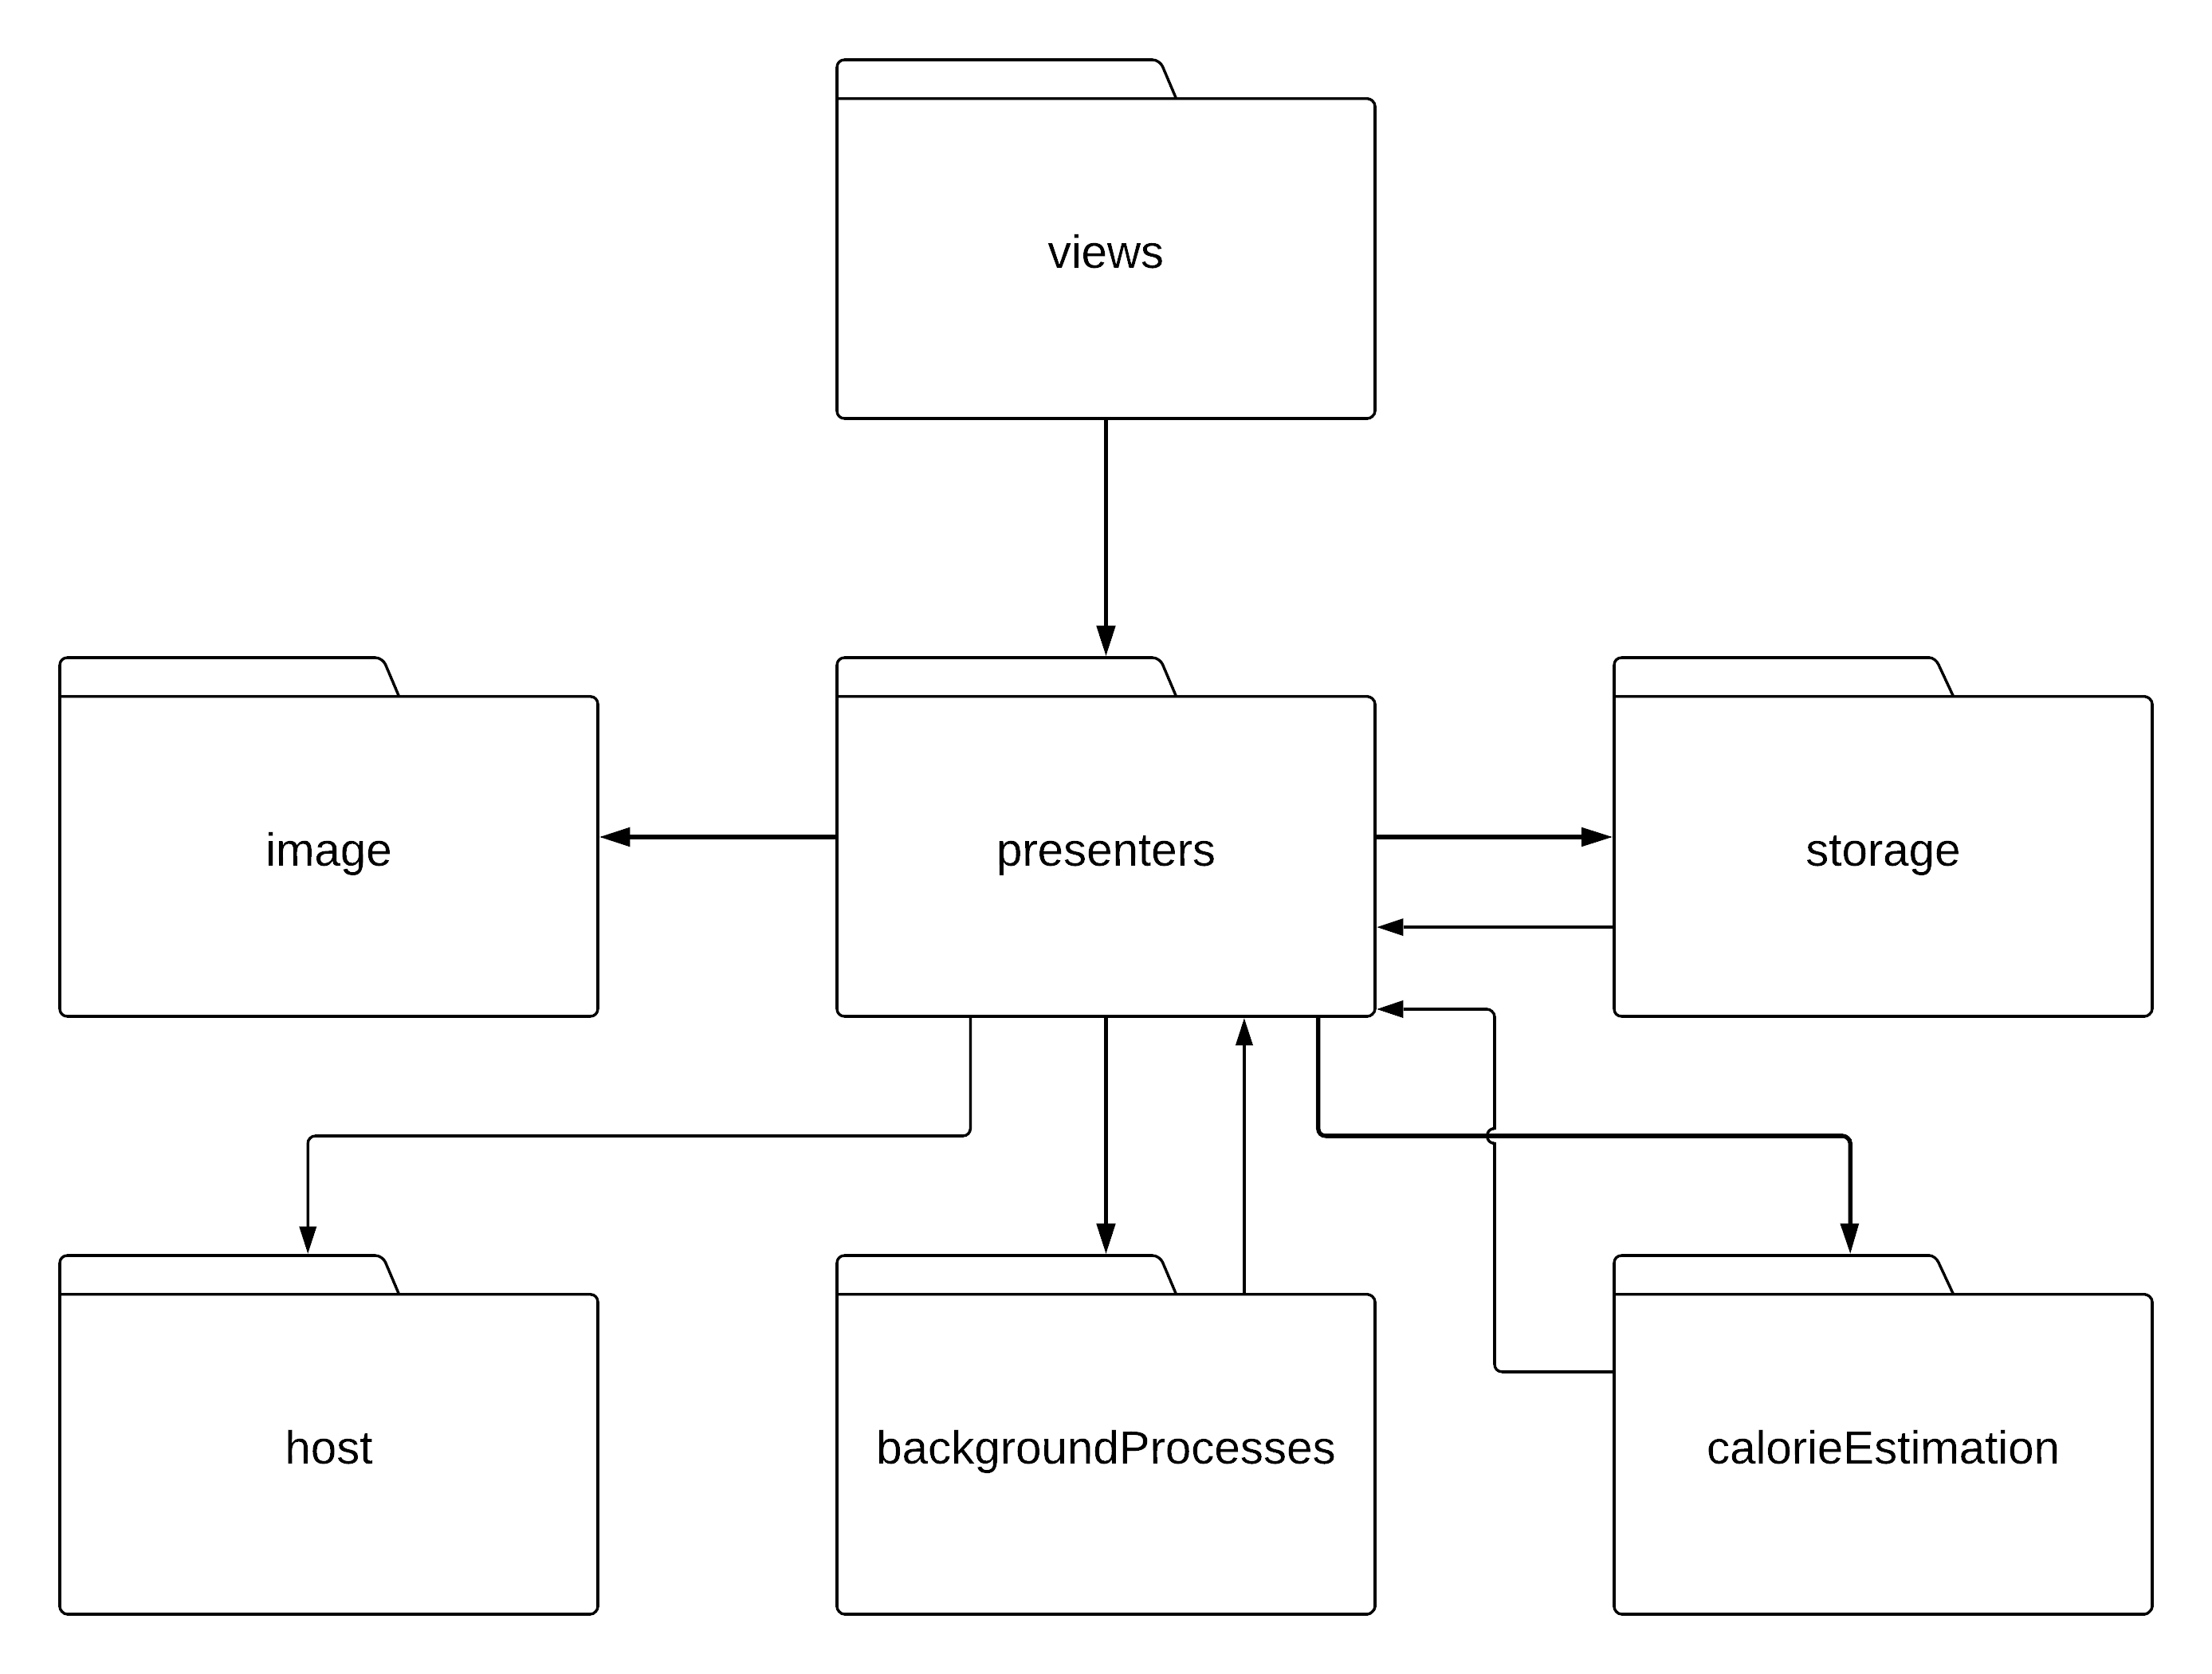
\includegraphics[scale=0.15]{packageDiagram}
    \caption{Package Diagram}
    \label{fig:packageDiagram}
\end{figure}

\subsubsection*{Architectural Patterns}
The Model-View-Presenter (MVP) architectural pattern was adapted for this application \parencite{mvp}.
This pattern is very similar to the Model-View-Controller (MVC) architecture which is quite popular in the software development industry.
The main difference between MVC and MVP is that whereas in MVC the controller is responsible for which view is used, in MPV the presenter is called through the view.
This is due to the architecture of Android applications in general, where the view takes primary control.
In the view classes, there should be no logic whatsoever in an MVP architecture and all logic should be called in the presenters.
There is also a one to one dependency between views and presenters.

As illustrated in Figure \ref{fig:packageDiagram}, the views in the application
have a dependency only on their corresponding presenter.
The presenters contain the business logic of the  application and have a dependency on all other packages.
The packages of backgroundProcesses, calorieEstimation and storage have a dependancy on the presenters package for callback purposes and also database creation in Android requires context of the activity information.

\subsubsection*{Marchitecture}
In Figure \ref{fig:market}, a marchitecture diagram can be seen.
This diagram represents the architecture of the system.
NutriLog is an Android application that send an image to an AWS (Amazon Web Services) instance using the API OkHttp. The AWS instance is running a Python FLASK application that classifies the image using a TensorFlow model and sends a response back to NutriLog. The Nutritionix API is used to collect nutritional information of this classification.

\begin{figure}[h]
    \centering
    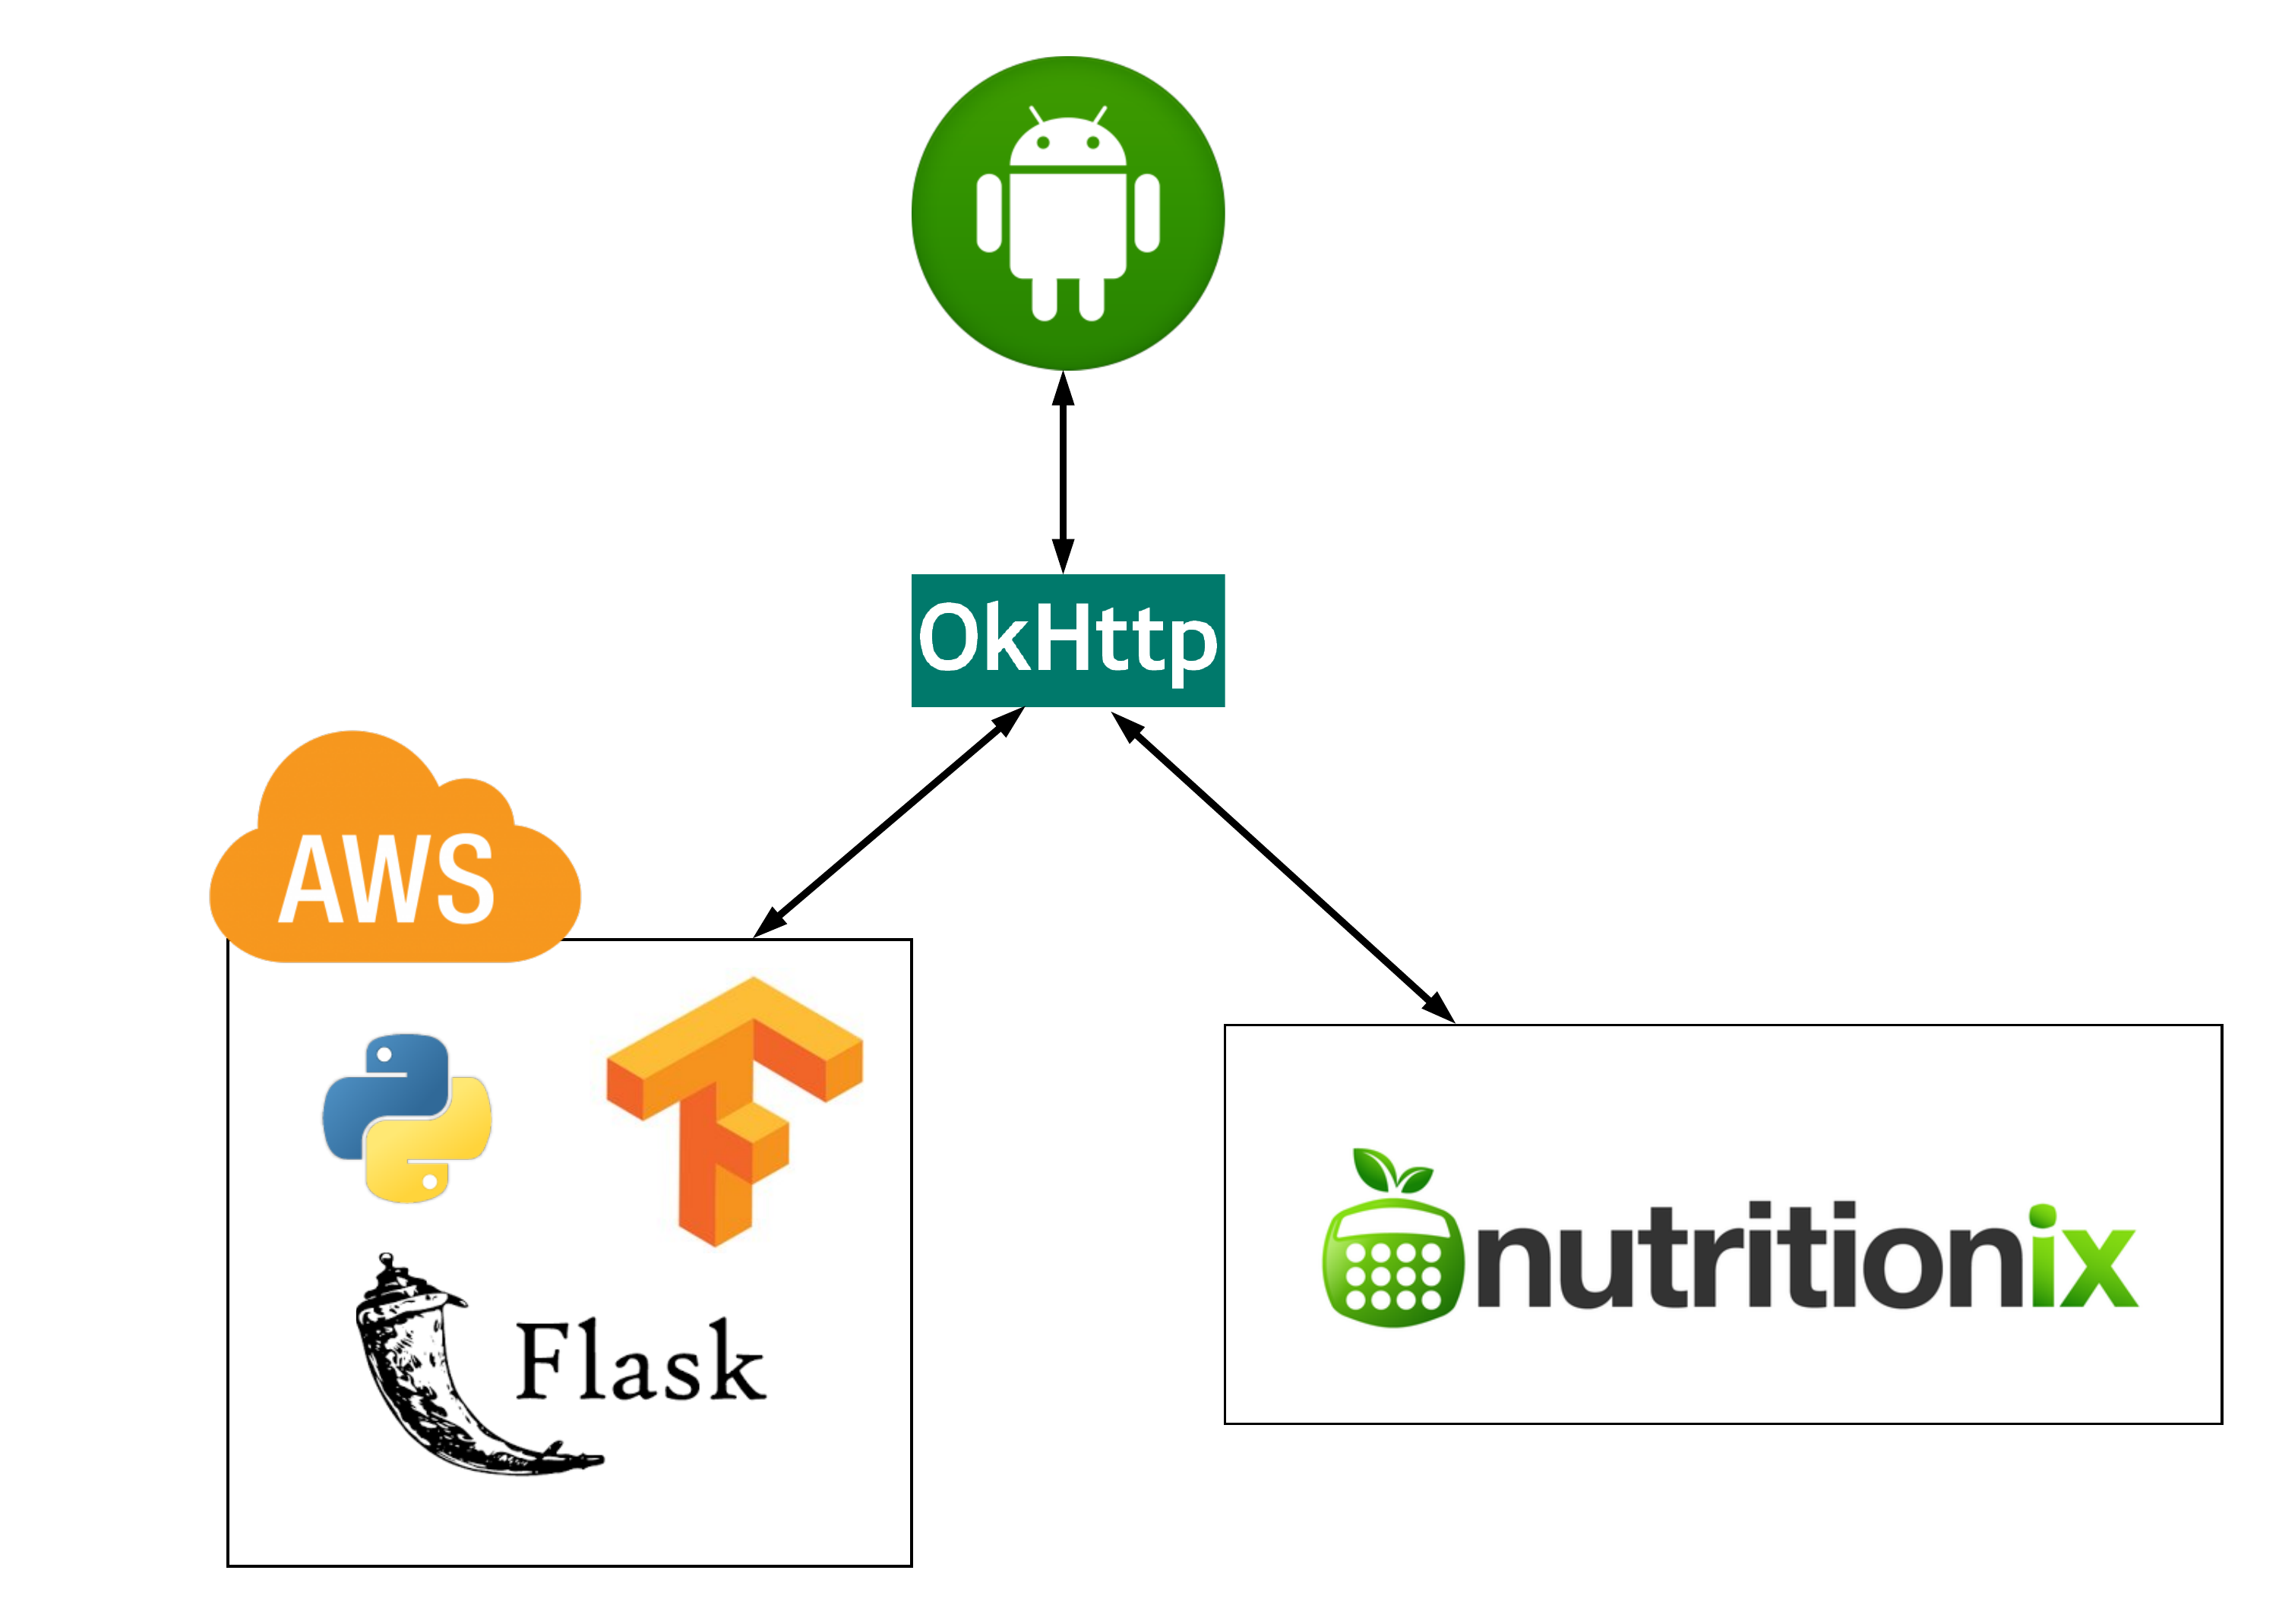
\includegraphics[scale=0.15]{market}
    \caption{Marchitecture Diagram}
    \label{fig:market}
\end{figure}

The technologies used for this appliction were used for the following reasons:

\textbf{AWS}
\linebreak
Past experience was a large factor when it came to choosing a cloud provider to host the backend instance for this prototype application.
AWS instances are very easy to set up once the process has been carried out a few times and this was a contributing factror to why AWS was chosen.
AWS also has a free tier which provides all the necessary server space to host the backend service for this application.

\textbf{OkHttp}
\linebreak
OkHttp seemed to be popular for Android applications as seen on websites such as Stack Overflow.
OkHttp also has extensive documentation and is a very simple API to import into Android.
The learning curve for OkHttp is quite small and it doesn't require much code to carry out a simple task like sending a HTTP POST request to a backend instance.

\textbf{FLASK}
\linebreak
Python FLASK was used for the backend service in this FYP due to past experience and its simplicity.

\textbf{TensorFlow}
\linebreak
TensorFlow was chosen as the library to create neural networks for this FYP mostly because of its reputation.
TensorFlow has been used by many researches in the computer vision industry.
TensirFlow also has extensive documentation and a wide array or resources and tutorials.

\textbf{Nutritionix}
\linebreak
Nutrionix was the best nutrional information API that was also free to use and this is why it was chosen.